%======================================================================
\subsection{SNC Subsystem Concept Definition}
\label{subsec:snc-concept-definition}
%======================================================================

The \gls{snc} subsystem implements centralized coordination, navigation decision-making, and operator interaction for the \gls{marv} platform. The design employs hierarchical state-machine architecture with separation of concerns. State management is decoupled from navigation logic. The design implements deterministic transitions, \gls{hub} compatibility for testability, \gls{sos} override capability, and \gls{scs} protocol compliance.

%----------------------------------------------------------------------
\subsubsection{Operational Concept}

System operation follows a four-state sequence: IDLE initialization, CAL calibration with dual \gls{eoc} assertion, MAZE autonomous navigation with \gls{navcon} logic, and \gls{sos} operator safety override via 2800~Hz dual-tone detection. Touch activation triggers IDLE$\rightarrow$CAL, dual \gls{eoc} enables CAL$\rightarrow$MAZE, \gls{eom} returns MAZE$\rightarrow$IDLE, and dual-tone toggles MAZE$\leftrightarrow$\gls{sos}.

\begin{figure}[H]
\centering
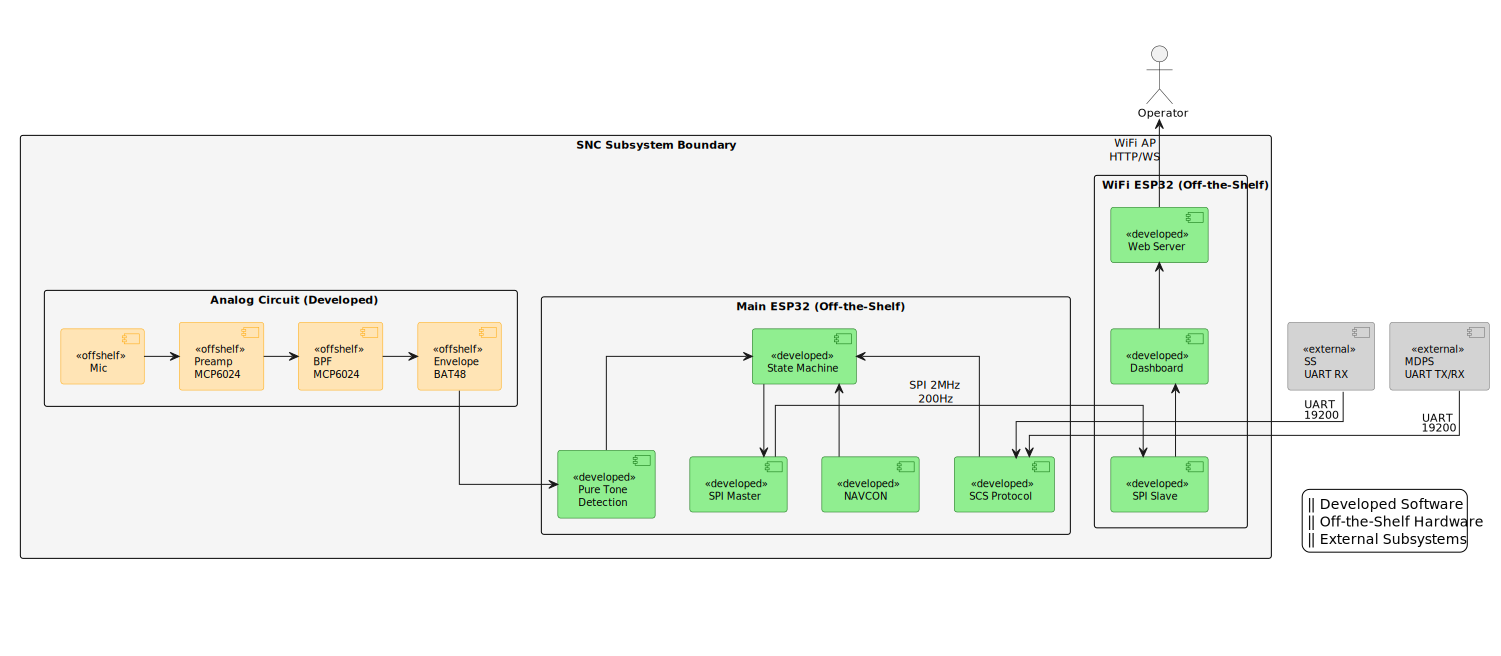
\includegraphics[width=1.05\textwidth]{01_SNC/diagrams/snc_architecture/out/snc_architecture.pdf}
\caption{\gls{snc} Architecture showing hardware and software with developed components in green, off-the-shelf in orange. Main ESP32 executes control, WiFi ESP32 handles telemetry, analogue circuit detects tones.}
\label{fig:snc-architecture-hw-sw}
\end{figure}

%----------------------------------------------------------------------
\subsubsection{Architecture Overview}

Figure~\ref{fig:snc-architecture} presents the \gls{snc} subsystem functional block diagram showing layered architecture with component interactions and data flows.

\begin{figure}[H]
\centering
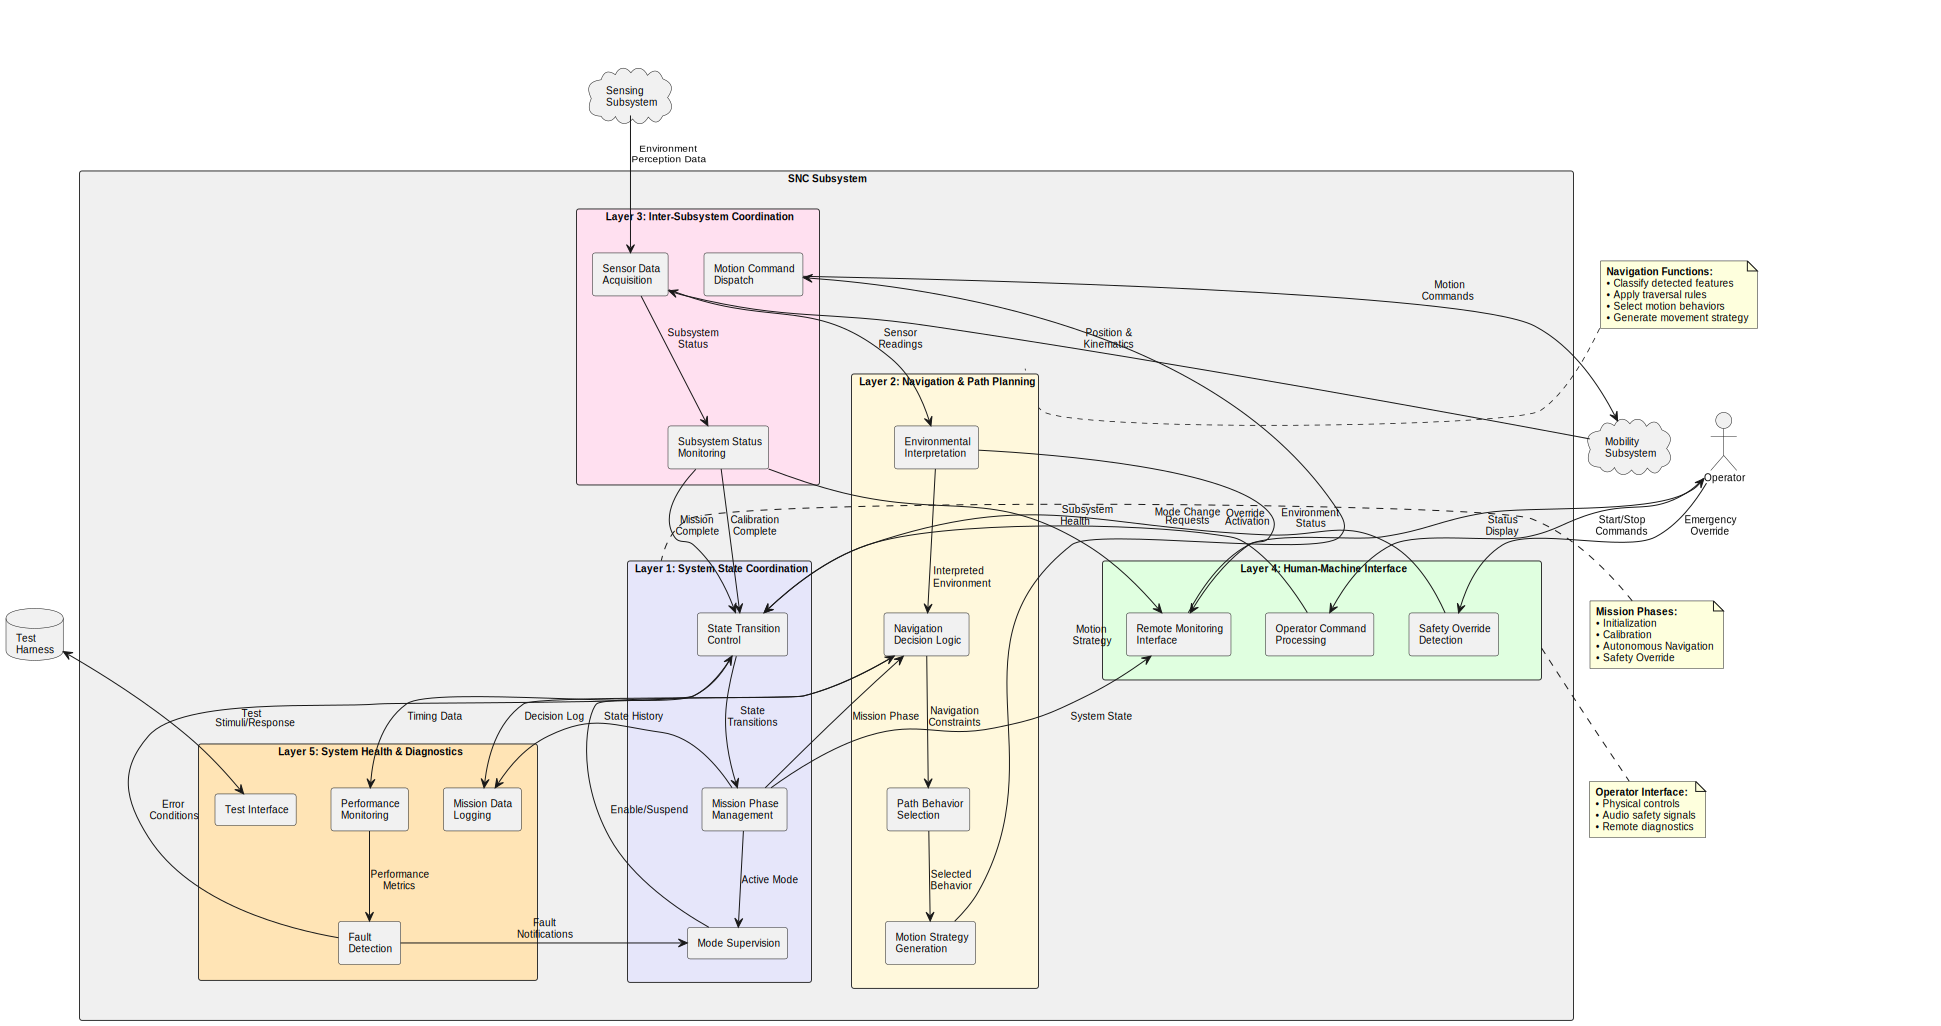
\includegraphics[width=0.98\textwidth]{01_SNC/diagrams/architecture_block/out/architecture_block.pdf}
\caption{\gls{snc} Subsystem Functional Block Diagram showing layered architecture: State Management, Navigation Decision, Communication Protocol, Touch/Tone Input, and Supervision \& Diagnostics.}
\label{fig:snc-architecture}
\end{figure}

The hardware comprises Main ESP32 managing state machine, \gls{navcon}, \gls{scs} protocol, touch sensor, and tone GPIO. WiFi ESP32 handles web server, telemetry dashboard, and \gls{spi} slave interface. The Pure Tone Circuit includes microphone, preamplifier, 4th-order 2800~Hz bandpass filter, envelope detector, and comparator. Capacitive Touch uses ESP32 TOUCH pin with 50~ms debouncing.

Software components include the State Machine implementing IDLE, CAL, MAZE, and \gls{sos} with guard conditions. NAVCON Logic applies angle-dependent navigation rules. The SCS Protocol Stack operates at UART 19200 baud with 4-byte packets. SPI Telemetry transmits at 200~Hz to WiFi ESP32 using 257-byte packets with DMA. The Web Dashboard uses HTML5 and JavaScript interface for real-time diagnostics.

External interfaces connect via UART at 19200 baud to \gls{ss} for RX and \gls{mdps} for TX and RX per \gls{scs} specification. Internal \gls{spi} at 2~MHz links Main and WiFi ESP32 with 200~Hz telemetry. WiFi AP operates at 192.168.4.1 with HTTP server on port 80 and WebSocket on port 81. Capacitive touch and tone circuit GPIO connect to Main ESP32.

%======================================================================
